\chapter{Efficient Incremental Search}
\label{chap:ibid}

In Chapter~\ref{chap:lazysp},
we introduced the Lazy Shortest Path (LazySP) algorithm,
which addresses domains with expensive edge weight functions
by interleaving the evaluation phase with a sequence of 
search queries using an existing pathfinding algorithm.
Because this inner search is conducted many times,
its efficiency is paramount.

Most approaches for reducing the computational cost of pathfinding
attempt to focus the search on a smaller subset of the graph.
We consider three classes of such techniques
(Figure~\ref{fig:ibid:intro-focus}):

\begin{marginfigure}[5cm]%
   \centering%
   \subfloat[Bidirectional search.]{%
      \centering %
      \includegraphics{build/ibid-intro-focus-bidirectional} %
   }%
   
   \subfloat[Heuristic search.]{%
      \centering %
      \includegraphics{build/ibid-intro-focus-heuristic} %
   }%
   
   \subfloat[Incremental search.]{%
      \centering %
      \includegraphics{build/ibid-intro-focus-incremental} %
   }%
   
   \caption{Illustrations of the three focusing techniques considered
      on a spatial pathfinding problem.}%
   \label{fig:ibid:intro-focus}
\end{marginfigure}

\begin{enumerate}
\item \emph{Bidirectional Search} -- A bidirectional algorithm
   conducts two concurrent searches,
   one from the source vertex $s$,
   and the other from the sink vertex $t$.
   Such searches are well-suited to roadmaps in ambient spaces that
   are high-dimensional and/or have
   obstacles situated close to the source/sink vertices.
\item \emph{Heuristic Search} -- A heuristic-informed algorithm
   exploits a sink-directed heuristic function over vertices to bias
   exploration in the direction of the sink vertex.
   A strong and admissible such heuristic can drastically speed the
   search,
   although the efficacy is reduced for weaker heuristics.
\item \emph{Incremental Search} -- An incremental algorithm
   is applied to a sequence of search queries on a graph whose
   edge weight function changes (partially) between queries.
   It endeavors to only consider the portion of its data structure
   affected by the changes.
\end{enumerate}

The principal contribution of this chapter is IBiD,
an algorithm which combines these three techniques into a single
algorithm
(Table~\ref{tab:ibid:alg-overview}).
While originally motivated for use with LazySP,
IBiD is broadly applicable to incremental search problems.

\paragraph{Chapter outline.}
In Section~\ref{sec:ibid:distance-functions},
we review distance functions and unidirectional methods.
Section~\ref{sec:ibid:bidirectional} reviews
bidirectional search methods.
In Section~\ref{sec:ibid:incremental},
we review incremental search
and introduce IBiD,
an algorithm which combines bidirectional and incremental search.
In Section~\ref{sec:ibid:heuristic},
we review heuristic search methods,
and discuss a heuristic-informed generalization of IBiD.
The chapter concludes with experimental results and implentation notes.

\begin{table}
   \centering
   \begin{tabular}{ccc}
      \toprule
      & Unidirectional & Bidirectional \\
      \midrule
      \addlinespace[0.2em]
      Complete
         & Dijkstra \citep{dijkstra1959anote}
         & Bidirectional Dijkstra \citep{luby1989bidijk} \\
      \addlinespace[-0.2em]
      \emph{(Heuristic)}
         & \emph{A* \citep{hart1968astar}}
         & \emph{Bidirectional A* \citep{ikeda1994betterroutes}} \\
      \addlinespace[0.3em]
      Incremental
         & DynamicSWSF-FP \citep{ramalingam1996dynamicswsffp}
         & {IBiD} \\
      \addlinespace[-0.2em]
      \emph{(Heuristic)}
         & \emph{Lifelong Planning A* \citep{koenig2004lpastar}}
         & \emph{Heuristic IBiD} \\
      \addlinespace[0.2em]
      \bottomrule
   \end{tabular}
   \caption{
      IBiD generalizes both the heuristic-informed
      bidirectional Dijkstra's search \citep{goldberg2005spexternalmemory}
      and DynamicSWSF-FP \citep{ramalingam1996dynamicswsffp}.
      There are a great many algorithms that we could place in each cell;
      we provide only a represetative choice in each.}
   \label{tab:ibid:alg-overview}
\end{table}

\section{Search via Distance Functions}
\label{sec:ibid:distance-functions}

\paragraph{Problem definition.}
The \emph{shortest path problem} on graphs has been extensively
studied over the past six decades.
Consider a directed graph $G = (V,E)$ and accompanying edge weight
function $w : E \rightarrow \mathbb{R}$,
with the length of a path equal to the sum of the weights of its
constituent edges.
\marginnote{
The single-pair problem is also called the \emph{two-terminal} or
\emph{point-to-point} problem.}
I include here a brief survey of algorithmic work on the
\emph{single-pair shortest path} (SPSP) problem,
where a path of minimal length is sought
between distinct source and target vertices
$s,t \in V$.
I also consider only graphs without negative-length cycles.
Note that we can also handle planning problems with multiple
start/goal configurations as an SPSP problem
as described in Section~\ref{subsec:roadmaps:planning-as-pathfinding}.

\paragraph{An example problem.}
\begin{marginfigure}%
   \centering%
   \begin{tikzpicture}
      \tikzset{>=latex} % arrow heads
      \node[inner sep=0pt,anchor=south west] {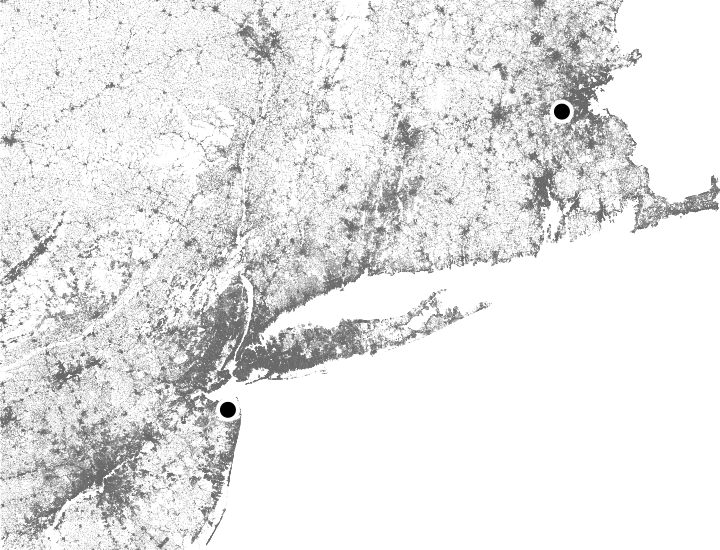
\includegraphics[width=5cm]{figs/incbi-road-ne/singleshot/example-intro.png}};
      \coordinate (s) at (1.75,0.9);
      \coordinate (t) at (3.93,2.8);
      \node (slab) at (2.5,0.6) {$s$};
      \node (tlab) at (4.0,1.5) {$t$};
      \draw[->,thick] (slab) -- (s);
      \draw[->,thick] (tlab) -- (t);
   \end{tikzpicture}%
   \caption{A graph of the Northeast USA from the 9th DIMACS
      Implementation Challenge
      comprises 1,524,453 vertices and 3,868,020 directed edges.
      A shortest path problem from a source $s$ in New Jersey
      to a target $t$ outisde Boston
      will be used as an example.}%
   \label{fig:ibid:example-intro}%
\end{marginfigure}
We will carry forward an illustrative example problem from
the public dataset of the 9th DIMACS Implementation Challenge
\citep{demetrescuetal2006dimacs9}
(Northeast USA)
comprising an approximate road network,
using transit time as the edge weight function
(Figure~\ref{fig:ibid:example-intro}).
In this way,
a shortest path between a pair of sink and target locations
minimizes the total transit time between them.

\paragraph{Problem Settings.}
The single-pair problem has been extensively studied.
There are techniques that are particular to memory-constrained
settings \citep{kaindl1997biheurreconsidered}
or to settings where pre-computation is available
\citep{goldberg2007pointtopoint}.
While we do not focus on such settings,
the algorithm we propose is complementary to these techniques.

\subsection{Pathfinding via the Source Distance Function}

The pioneering pathfinding algorithms of the late 1950s address
a generalization of the SPSP problem called
the \emph{single-source} problem,
where shortest paths are calculated from $s$ to all vertices on
the graph.
They proceed by calculating the \emph{source distance function}
$d^* : V \rightarrow \mathbb{R}$,
which gives the length of the shortest path from $s$
to each vertex $v$.
In other words:
\marginnote{Once the distance function $d^*$ is computed,
a shortest path to any target $t$ can be generated trivially
by walking backwards to $s$ guided by $d^*$.}
\begin{equation}
   d^*(v) = \min_{p \in P_{sv}} \mbox{len}(p),
   \label{eqn:ibid-distance-function-global}
\end{equation}
where $P_{sv}$ is the set of all paths from $s$ to $v$.
Where no paths to $v$ exist,
we take $d^*(v) = \infty$.
Note that $d^*$ is only well-defined on graphs with no negative-length
cycles reachable from $s$.

\begin{marginfigure}%
   \centering%
   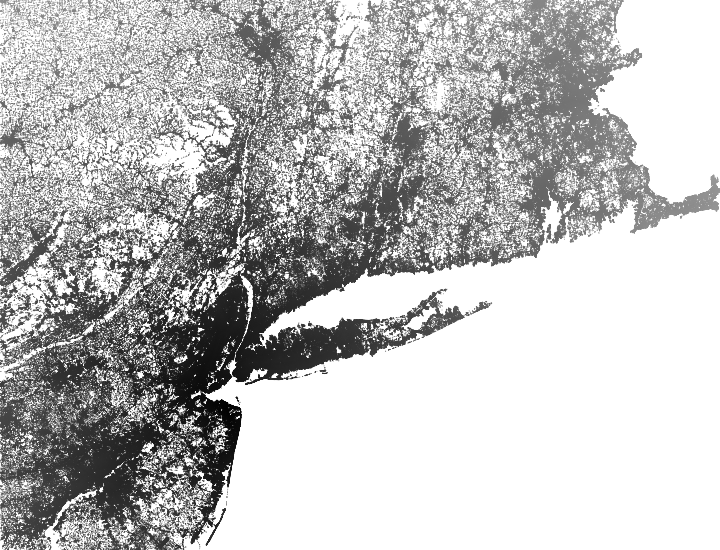
\includegraphics[width=5cm]{figs/incbi-road-ne/singleshot/example-dijkstraall.png}%
   \caption{The distance function from the source vertex.}%
   \label{fig:ibid:example-distance-all}%
\end{marginfigure}

Importantly, $d^*$ can also be characterized locally by
\begin{equation}
   d^*(v) = 
   \left\{ \begin{array}{cl}
      0 & \mbox{if } v = s \\
      \displaystyle\min_{u \in \mbox{\scriptsize Pred}(v)} d^*(u) + w(u,v) & \mbox{otherwise,} \\
   \end{array} \right.
   \label{eqn:distance-function-char}
\end{equation}
where $\mbox{Pred}(v)$ yeilds the predecessor vertices
of $v$.
\marginnote{Note that
while the distance function $d^*$ necessarily satisfies
the equations (\ref{eqn:distance-function-char}),
they are not generally a sufficint condition;
if a reachable cycle of zero length exists,
(\ref{eqn:distance-function-char}) will not have a unique solution.}
The distance function is akin to the \emph{value function}
in more general decision problems addressed by dynamic programming.
The equations (\ref{eqn:distance-function-char})
are the \emph{Bellman equations} \citep{bellman1958routing},
which rely on the principle of optimality.
This characterization also follows implicitly from early results for
the all-pairs problem
\citep{shimbel1955communicationnets, beckmann1955transportation}.
Note that (\ref{eqn:distance-function-char}) is a necessary condition
of $d^*$,
it is not sufficient in general.
In particular,
if $w$ has cycles of zero length,
there will be multiple solutions of (\ref{eqn:distance-function-char})
which are not the well-defined $d^*$.

\paragraph{Reconstructing a Shortest Path from the Distance Function}
\cdnote{Add note about path reconstruction.
Problem if there exist zero-length cycles.}

\subsection{Approximating $d^*$ via Tensioned Estimates}
\label{subsec:ibid-tension}

How can we compute $d^*$ efficently over the graph?
Consider an approximation function $d$
which satisfies the following properties:
\begin{subequations}%
   \begin{eqnarray}
      & d^*(v) \leq d(v) & \forall v \in V
         \label{eqn:ibid-relaxation-props-nounder} \\
      & d(s) = 0 &
         \label{eqn:ibid-relaxation-props-ds0} \\
      & d(u) + w(e_{uv}) \geq d(v) & \forall e_{uv} \in E
         \label{eqn:ibid-relaxation-props-tens}
   \end{eqnarray}%
   \label{eqn:ibid-relaxation-props}%
\end{subequations}%

\begin{theorem}
If $d: V \rightarrow \mathbb{R}$
satisfies (\ref{eqn:ibid-relaxation-props}),
then $d = d^*$.
\label{thm:ibid-relaxation-notension}
\end{theorem}

\begin{proof}[Proof of Theorem~\ref{thm:ibid-relaxation-notension}]
Consider any vertex $x$.
If $d^*(x) = \infty$,
then by (\ref{eqn:ibid-relaxation-props-nounder}) we must have that
$d(x) = \infty$.
Otherwise,
by (\ref{eqn:ibid-distance-function-global}),
there exists a path $p^*$ of length $d^*(x)$;
consider this path.
The first vertex on $p^*$ is $s$ with $d^*(s) = 0$,
and by (\ref{eqn:ibid-relaxation-props}),
$d(s) = d^*(s)$.
For each edge $e_{uv}$ on $p^*$ with $d(u) = d^*(u)$,
we will show that $d(v) = d^*(v)$.
By definition of the shortest path,
$d^*(u) + w(e_{uv}) = d^*(v)$.
Therefore $d(u) + w(e_{uv}) = d^*(v)$,
and by (\ref{eqn:ibid-relaxation-props-tens}),
we have $d^*(v) \geq d(v)$,
and by (\ref{eqn:ibid-relaxation-props-nounder})
we have $d^*(v) = d(v)$.
By induction along the path $p^*$,
we have that $d(x) = d^*(x)$.
\end{proof}

\subsection{Tensioned Estimates and Edge Relaxation}

The principal method for arriving at an approximation
which satisfies (\ref{eqn:ibid-relaxation-props})
is via \emph{tensioned estimates}.
Consider the following labeling on an arbitrary approximation $d$:
\begin{equation}
   \mbox{edge } e_{uv} \mbox{ is \emph{tensioned}}
   \;\;\mbox{iff}\;\;
   d(u) + w(e_{uv}) < d(v).
   \label{eqn:ibid-relaxation-tensioned}
\end{equation}
Tensioned edges are therefore those that violate
(\ref{eqn:ibid-relaxation-props-tens}).
A restatement of Theorem~\ref{thm:ibid-relaxation-notension}
is that an approximation $d$
satisfying (\ref{eqn:ibid-relaxation-props-ds0})
and (\ref{eqn:ibid-relaxation-props-nounder})
with no tensioned edges is everywhere correct.

How can we arrive at an approximation
satisfying Theorem~\ref{thm:ibid-relaxation-notension}?
We can initialize a $d$ so as to trivially
satisfy (\ref{eqn:ibid-relaxation-props-ds0})
and (\ref{eqn:ibid-relaxation-props-nounder}),
such as $d(v) = \infty \;\forall v \neq s$,
which will generally have many edges in tension.
The principal technique for improving $d$ relies on the principle of
\emph{relaxation}
as described by Ford \citep{ford1955networkflowtheory}.
An algorithm can iteratively select a tensioned edge $e_{uv}$
and relax it by setting
$d(v) \leftarrow d(u) + w(e_{uv})$.
It can be shown that applying this process arbitrarily
maintains the properties in (\ref{eqn:ibid-relaxation-props}).

It can be further shown that for a finite graph,
the number of edge relaxations needed is also finite.
The well-known Bellman-Ford method
\citep{shimbel1955communicationnets, bellman1958routing,
moore1959spmaze}
cycles through all edges repeatedly,
relaxing all tensioned edges found
(at most $|V|-1$ repetitions are sufficient for convergence).
Note that this does not place any requirements on $G$
(other than that $d^*$ must exist, so there must not be
any negative-length cycles reachable from $s$).

\subsection{Soundness, Trust Regions, and an Efficient Ordering}

The need for multiple cycles of Bellman-Ford stems from the fact
that each edge may need to be relaxed several times.
Consider the vertices $a \rightarrow b \rightarrow c$,
with edges $e_{ab}$ and $e_{bc}$ both in tension;
if $e_{bc}$ is relaxed before $e_{ab}$,
then $e_{bc}$ will need to be relaxed a second time.
This occurrs because relaxing an edge changes the
$d$-value of the target vertex,
which may newly tension downstream edges.

We can exploit our intution to order relaxations from source to sink
in the special case where $w \geq 0$
(note that this requirement is stronger than requiring no reachable
negative-length cycles).
We can show that our approximation $d$
is \emph{sound} for a subset of vertices
as described by Theorem~\ref{thm:ibid-relaxation-sound}.

\begin{marginfigure}
   \centering
   \includegraphics{build/ibid-dijkstra-trust}
   \caption{Tensioned edge trust region
      for $w \geq 0$.
      Contours are of the current estimate $d$.
      Currently tensioned edges are bold and dotted.}
\end{marginfigure}

\begin{theorem}
Let $d'$ be the smallest value $d(u)$
for any edge $e_{uv}$ labeled as in tension
by (\ref{eqn:ibid-relaxation-tensioned}).
If $w \geq 0$,
any vertex $v$ with $d(v) \leq d'$
has $d(v) = d^*(v)$.
\label{thm:ibid-relaxation-sound}
\end{theorem}

\begin{proof}[Proof of Theorem~\ref{thm:ibid-relaxation-sound}]
The proof proceeds as follows.
First, if $d' = \infty$,
then no edges can be in tension,
and so $d = d^*$ everywhere
as shown in Section~\ref{subsec:ibid-tension}.
Otherwise,
suppose that $d(x) \neq d^*(x)$
for some vertex $x$ with $d(x) \leq d'$.
By (\ref{eqn:ibid-relaxation-props}),
it would have to be that $d^*(x) < d(x)$.
Consider a true shortest path $p$ from $s$ to $x$;
by (\ref{eqn:ibid-relaxation-props})
such a path exists and has finite length $d^*(x)$.
By (\ref{eqn:ibid-relaxation-props}),
we have that $d^*(s) = d(s) = 0$
(and so $s$ and $x$ must be distinct).
Let $e_{uv}$ be the first edge along $p$ such that
$d^*(u) = d(u)$
but $d^*(v) < d(v)$.
Since $p$ is a shortest path,
edge $e_{uv}$ must therefore be in tension.
Since $w \geq 0$,
it must be that $d^*(u) \leq d^*(x)$;
further, since $d^*(u) = d(u)$,
$d^*(x) < d(x)$,
and $d(x) \leq d'$
it must be that $d(u) < d'$.
But then edge $e_{uv}$ is in tension with lower $d(u)$!
This contradiction implies that every vertex $x$
with $d(x) \leq d'$
must have $d(x) = d^*(x)$.
\end{proof}

As a result,
a given value $d'$ creates a region of vertices
with values $d(x) \leq d'$ that are known to be
accurate.
This confers two distinct advantages when designing an algorithm.
First,
all tensioned edges $e_{uv}$ with $d(u) = d'$
(of which there must be at least one if any edges are in tension)
can be relaxed immediately,
and will never be retensioned.
This is exactly the order imposed by the OPEN list in Dijkstra's
algorithm \citep{dijkstra1959anote}.

\subsection{Completeness and Early Termination}
\label{subsec:ibid-dijkstra-completeness}

\begin{marginfigure}%
   \centering%
   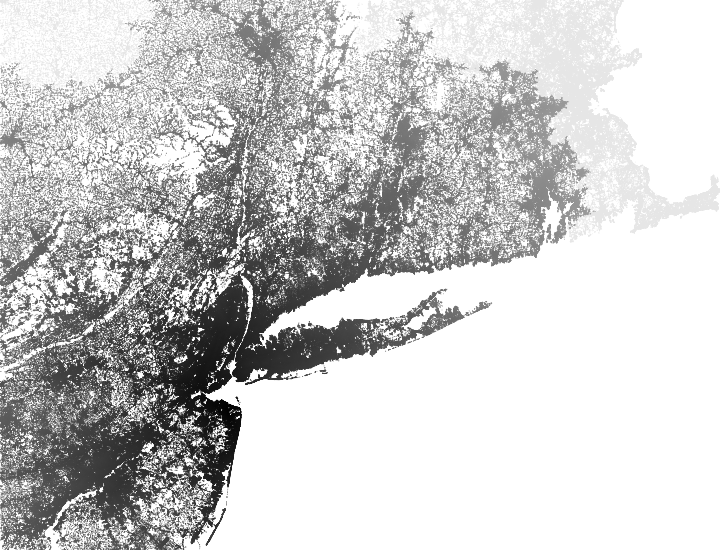
\includegraphics[width=5cm]{figs/incbi-road-ne/singleshot/example-dijkstra.png}%
   \caption{Dijkstra's algorithm computes the start distance function
      $d^*$ to solve the example shortest path problem.
      Darker vertices have smaller $d$-values.
      The algorithm stops upon reaching the target vertex $t$
      after expanding 1,290,820 vertices.}%
   \label{fig:ibid:example-distance}%
\end{marginfigure}

If a path is sought only a particular destination vertex $t$,
it is beneficial to terminate the algorithm before all edges are relaxed.
The soundness result (Theorem~\ref{thm:ibid-relaxation-sound})
demonstrates that once $d(t) \leq d'$,
the value $d(t)$ is known to be correct.
However,
proving that a back-reconstructed solution path is correct
requires a complementary completeness result --
that it, to show that if a better solution exists,
it would have been found.

Unfortunately the edge cases for completeness are less strong
than for soundness.
See the example in Figure~\ref{fig:ibid:relaxation-completeness-issue}.
\cdnote{Add note about how in the special case where $d$ is initialized
to $\infty$ and all $d$-values are thereafter reduced via edge
relaxations,
this completeness result also extends to the case of
$w \geq 0$ and $d^*(x) \leq d'$.
But this result isn't applicable to incremental settings as we'll
discuss in Section~\ref{sec:ibid:incremental}.}

\begin{marginfigure}
   \centering
   \begin{tikzpicture}
      \tikzset{>=latex} % arrow heads
      \node[fill=black,circle,inner sep=1.2pt] (s) at (0,0) {};
      \node[fill=black,circle,inner sep=1.2pt] (a) at (1.5,0) {};
      \node[fill=black,circle,inner sep=1.2pt] (b) at (1.5,1.2) {};
      \node[fill=black,circle,inner sep=1.2pt] (x) at (3.0,0) {};
      \draw[->,densely dashed] (s) -- (a) node[midway,fill=white,circle,inner sep=1pt] {0};
      \draw[->] (a) -- (x) node[midway,fill=white,circle,inner sep=1pt] {0};
      \draw[->] (s) -- (b) node[midway,fill=white,circle,inner sep=1pt] {1};
      \draw[->] (b) -- (x) node[midway,fill=white,circle,inner sep=1pt] {1};

      \node[above=0.05cm of s] {$s$};
      \node[above=0.05cm of a] {$a$};
      \node[below=0.05cm of b] {$b$};
      \node[above=0.05cm of x] {$x$};

      \node[below=0.05cm of s] {$d=0$};
      \node[below=0.05cm of a] {$d=3$};
      \node[above=0.35cm of b] {$d=1$};
      \node[below=0.05cm of x] {$d=0$};

      \node[below=0.35cm of s] {$d^*=0$};
      \node[below=0.35cm of a] {$d^*=0$};
      \node[above=0.05cm of b] {$d^*=1$};
      \node[below=0.35cm of x] {$d^*=0$};
   \end{tikzpicture}
   \caption{Problem case for pathfinding with distance functions.
      Here, $d$ satisfied a and c, with edge $e_{sa}$ tensioned,
      and $d' = 0$.
      While the approximation $d$ is \emph{sound} at $x$
      ($d(x)$ is correct),
      reconstructing a shortest path requires \emph{completeness}.}
   \label{fig:ibid:relaxation-completeness-issue}
\end{marginfigure}

\begin{theorem}
If either $w \geq 0$ and $d^*(x) < d'$,
or if $w > 0$ and $d^*(x) \leq d'$,
then $d(x) = d^*(x)$.
\label{thm:ibid-relaxation-complete}
\end{theorem}

\begin{proof}[Proof of Theorem~\ref{thm:ibid-relaxation-complete}]
Consider a true shortest path $p^*$ of length $d^*(x)$ from $s$ to $x$.
Due to our conditions,
all vertices $u$ before $x$ on $p^*$ have $d^*(u) < d'$.
By (\ref{eqn:ibid-relaxation-props}),
we have $d(s) = d^*(s) = 0$.
Consider each edge $e_{uv}$ in turn along $p^*$,
for which $d^*(u) + w(e_{uv}) = d^*(v)$.
For each, suppose that $d(u) = d^*(u)$.
Then we have $d(u) < d'$,
so that edge $e_{uv}$ must not be in tension.
Thus $d(v) \leq d(u) + w(e_{uv})$,
and by (\ref{eqn:ibid-relaxation-props}) we know $d(v) = d^*(v)$.
Therefore, we have $d(x) = d^*(s)$.
\end{proof}

\begin{theorem}
If either $w \geq 0$ and $d^*(x) < d'$,
or if $w > 0$ and $d^*(x) \leq d'$,
then a shortest path can be reconstructed backwards from $x$
by prepending the incoming edge $e_{uv}$ which minimizes
$d(u) + w(e_{uv})$ until $s$ is reached.
\label{thm:ibid-relaxation-reconstruct}
\end{theorem}

\begin{proof}[Proof of Theorem~\ref{thm:ibid-relaxation-reconstruct}]
We will show that for every such vertex $x$,
there exist a predecessor $u$ and incident edge $e_{uv}$
for which $d(u) + w(e_{uv}) = d(x)$.
It follows that $e_{uv}$ is on a shortest path to $x$.
This argument can then be applied recursively to $u$,
which must still satisfy the necessary conditions.
\end{proof}

\section{Bidirectional Search}
\label{sec:ibid:bidirectional}

One prominent technique for minimizing pathfinding computation for
single-pair problems
is bidirectional search.
In a bidirectional algorithm,
the distance $d_t$ to the target is calculated in a growing region
around the target vertex $t$
concurrently with the conventional source distance $d_s$ around $s$
(Figure~\ref{fig:ibid:example-bidirectional}).
Loosely speaking,
the search can terminate with a shortest path
once the two regions intersect.
The savings relative to a unidirectional search grow with the problem's
branching factor.
For roadmap graphs embedded in an ambient space,
this branching factor can be linear or exponential in the space's
dimension.
\begin{marginfigure}%
   \centering%
   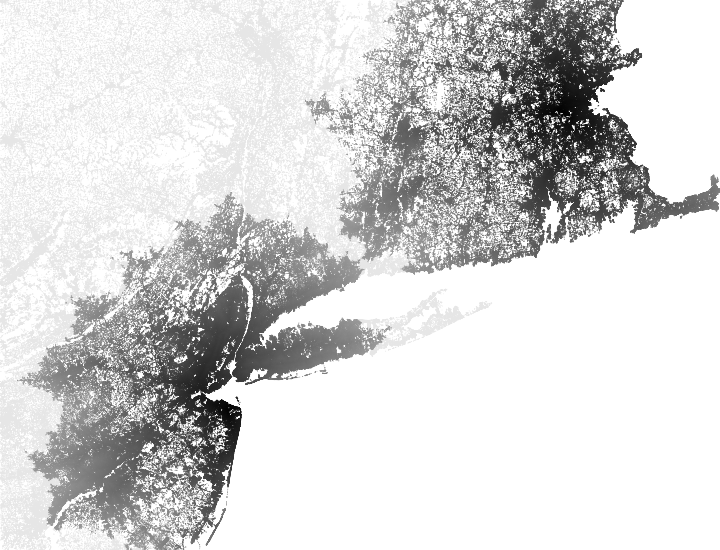
\includegraphics[width=5cm]{figs/incbi-road-ne/singleshot/example-bidijkstra.png}%
   \caption{The bidirectional Dijkatra's algorithm
      computes $d_s$ around the source vertex
      and $d_t$ around the target vertex.
      Darker vertices have smaller $d$-values in their respective
      regions.
      The algorithm terminates after expanding a total of
      1,178,200 vertices using distance to balance expansions.}%
   \label{fig:ibid:example-bidirectional}%
\end{marginfigure}

The first bidirectional algorithm
was proposed by Dantzig \citep{dantzig1963linearprogramming},
and the first precisely described algorithm was presented by
Nicholson \citep{nicholson1966shortest}.
Implementation of a sound and efficient algorithm
turns on two important questions:
(a) when and how to terminate with a shortest path,
and (b) how to balance expansions from the two directions of the
search.

\subsection{Termination Conditions}
\label{sec:ibid:bidirectional-termination}

What is the equivalent to the completeness-based termination condition
described in Section~\ref{subsec:ibid-dijkstra-completeness}?

What happens upon an encounter between the forward and reverse searches?
Goldberg \citep{goldberg2005spexternalmemory}
discusses the correct termination condition for the 
Bidirectional Dijkstra algorithm.

A correct termination condition is surprisingly subtle,%
\marginnote{There were early incorrect attempts at a sound
termination condition
\citep{berge1965programminggamestransportation}.}
with several correct variations proposed
\citep{nicholson1966shortest, dreyfus1969appraisalsp,
pohl1969bidirectional, goldberg2005spexternalmemory}.
The difficulty stems from the fact that the first vertex to be
{\sc Closed} by the searches in both directions
need not lie on the shortest path
(Figure~\ref{fig:ibid:bidirectional-termination-issue}).

Key point, reason about edges!

See Algorithm~\ref{alg:ibid:bidirectional-termination}.

\begin{algorithm}[t]
   \caption{Bidirectional Termination Condition}
   \label{alg:ibid:bidirectional-termination}
   \begin{algorithmic}[1]
      \State On $u$ expanded in the foward search
         with $v$ already expanded in the backward search,
   \end{algorithmic}
\end{algorithm}

\begin{marginfigure}
   \centering
   \begin{tikzpicture}
      \tikzset{>=latex} % arrow heads
      \node[fill=black,circle,inner sep=1.2pt] (s) at (0,0) {};
      \node[fill=black,circle,inner sep=1.2pt] (a) at (1.5,0) {};
      \node[fill=black,circle,inner sep=1.2pt] (b) at (3.0,0) {};
      \node[fill=black,circle,inner sep=1.2pt] (t) at (4.5,0) {};
      \node[fill=black,circle,inner sep=1.2pt] (c) at (2.25,0.8) {};
      \draw[->] (s) -- (a) node[midway,fill=white,circle,inner sep=1pt] {3};
      \draw[->] (a) -- (b) node[midway,fill=white,circle,inner sep=1pt] {3};
      \draw[->] (b) -- (t) node[midway,fill=white,circle,inner sep=1pt] {3};
      \draw[->] (a) -- (c) node[midway,fill=white,circle,inner sep=1pt] {2};
      \draw[->] (c) -- (b) node[midway,fill=white,circle,inner sep=1pt] {2};
      \node[below=0.05cm of s] {$s$};
      \node[below=0.05cm of a] {$a$};
      \node[below=0.05cm of b] {$b$};
      \node[below=0.05cm of t] {$t$};
      \node[above=0.05cm of c] {$c$};
   \end{tikzpicture}
   \caption{Simple illustration of a problem case for terminating
      a bidirectional search.
      With a balanced distance criterion,
      $c$ will be the first vertex expanded in both directions,
      but it does not lie on the shortest path.}
   \label{fig:ibid:bidirectional-termination-issue}
\end{marginfigure}

\subsection{Balancing Directions}
The general bidirectional algorithm leaves open the strategy
used to balance the progression of the two search directions.
Options based on alternating \citep{dantzig1963linearprogramming},
or selecting the direction with the smaller {\sc Open} distance
\citep{nicholson1966shortest}
or {\sc Open} (and finite) set cardinality
\citep{pohl1969bidirectional}
have been proposed.
Note that while some literature asserts that
these can be interleaved arbitrarily,
termination of the algorithm requires that each direction
be expanded at least once.
Our example problems use the balanced distance criterion.

\section{Incremental Search}
\label{sec:ibid:incremental}

How can we adapt the relaxation approach to the incremental setting?
And how can we recover the original algorithm from the more general one?

We can rely on just the consistency,
but not the upper bound part.
So now there are many solutions.
So we need to further constrain the graph to have
positive edge weights.

This stuff is more modern (1996, 2004).

A review is here: \citep{eppstein1999dynamic},
\citep{demetrescu2010dynamic}.

Talk about how this is centrally a restatement of the Dijktsra's ordering.
Bring in the invariant.

DynamicSWSF-FP \citep{ramalingam1996dynamicswsffp}.

How about this: \citep{frigioni2000dynamicsp}.

Revisit Bellman equation.

The central idea is that the search maintains the following invariant.
Note that this is a basic restatement of the distance function
ordering that underlies Dijkstra's algorithm.

Define $r$ and $d$,
what we mean by \emph{consistent},
and what $k$ is.

In general (no non-positive cycles),
the algorithm terminates.
The proof is that key values only increase (somehow).

All of the proofs in this section relate to
graphs with positive edge weights ($w > 0$),
with $k_{\ms{min}}$ the minimal key among inconsistent vertices.

\subsection{Approximation Soundness}

The theorems below are basically a soundness proof --
if our approximation yields values below a certain value,
they are known to be correct.
This is soundness of the approximation,
not of an algorithm per se.

\begin{theorem}
Any consistent vertex $x$ with $d[x] \leq k_{\ms{min}}$
has $d[x] = d^*(x)$.
\label{thm:ibid-dynamicswsffp-sound}
\end{theorem}

\begin{proof}[Proof of Theorem~\ref{thm:ibid-dynamicswsffp-sound}]
The proof relies upon a path construction described by
Lemma~\ref{lemma:ibid-dynamicswsffp-sound-conpath}.
We then show that $d[x]$ can be both
no less than $d^*(x)$
(Lemma~\ref{lemma:ibid-dynamicswsffp-sound-geq})
and no greater than $d^*(x)$
(Lemma~\ref{lemma:ibid-dynamicswsffp-sound-leq}).
\end{proof}

\begin{lemma}
For any consistent vertex $x$ with $d[x] \leq k_{\ms{min}}$,
there exists a path $p$ from $s$ to $x$
in which each vertex is consistent
and each edge $e_{uv}$ satisfies $d[u] + w(e_{uv}) = d[v]$.
\label{lemma:ibid-dynamicswsffp-sound-conpath}
\end{lemma}

\begin{proof}[Proof of Lemma~\ref{lemma:ibid-dynamicswsffp-sound-conpath}]
Construct the path $p$ as follows.
Initialize the path with the single vertex $x$.
Iteratively consider the first vertex $v$ on the path,
which is known to be consistent.
In the first case, if $v \neq s$,
then there exists a predecessor vertex $u$ and edge $e_{uv}$
with $d[u] + w(e_{uv}) = r(v)$.
Since $w > 0$ and $d[v] = r(v)$,
we have $d[u] < d[v] \leq d[x]$.
As a consequence,
$u$ is consistent;
prepend to the path the vertex $u$ and the edge $e_{uv}$,
and iterate.
In the second case, if $v = s$,
then we finish our construction of $p$.
Since the values $d[u]$ decrease monotonically
for all inserted vertices,
this process will terminate with a path $p$ beginning at $s$.
\end{proof}

\begin{lemma}
Any consistent vertex $x$ with $d[x] \leq k_{\ms{min}}$
has $d[x] \geq d^*(x)$.
\label{lemma:ibid-dynamicswsffp-sound-geq}
\end{lemma}

\begin{proof}[Proof of Lemma~\ref{lemma:ibid-dynamicswsffp-sound-geq}]
This follows directly from
Lemma~\ref{lemma:ibid-dynamicswsffp-sound-conpath}.
Since all vertices on the path are known consistent,
we must have $d[s] = 0$.
Further,
since the $d$-values across each edge in $p$
satisfy $d[u] + w(e_{uv}) = d[v]$,
it follows that $d[x] = \sum_{e \in p} w(e)$.
Therefore,
a path exists from $s$ to $x$ of length $d[x]$,
and so the true distance $d^*(x)$ must be upper-bounded by $d[x]$.
\end{proof}

\begin{lemma}
Any consistent vertex $v$ with $d[x] \leq k_{\ms{min}}$
has $d[x] \leq d^*(x)$.
\label{lemma:ibid-dynamicswsffp-sound-leq}
\end{lemma}

\begin{proof}[Proof of Lemma~\ref{lemma:ibid-dynamicswsffp-sound-leq}]
We demonstrate that $d[x] \leq d^*(x)$ by contradiction.
Suppose a vertex $x$ exists for which $d^*(x) < d[x]$.
Then there must exist a path $p'$ from $s$ to $x$ of length $d^*(x)$,
with $d^*(s) = 0$ and $d^*(u) + w(e_{uv}) = d^*(v)$ for each edge
in $p'$;
as a consequence,
we must have $d^*(v) < d[x]$ for all vertices $v$ on $p'$.
By Lemma~\ref{lemma:ibid-dynamicswsffp-sound-conpath},
we know that $s$ is consistent,
so $d[s] = 0$.
We will show that walking along
each edge $e_{uv}$ on $p'$ starting at $s$,
if $d[u] \leq d^*(u)$,
then $d[v] \leq d^*(v)$.

By definition,
we have $d[u] + w(e_{uv}) \geq r[v]$,
so that $d[u] - d^*(u) \geq r[v] - d^*(v)$.
Therefore,
it follows that $r[v] \leq d^*(v)$.
Since $k[v] \leq d^*(v)$,
it follows that $v$ is consistent,
so $d[v] \leq d^*(v)$.
We can replicate this logic down the path.
As a result,
it follows that $d[x] \leq d^*(x)$.
But this contraducts our supposition that $d^*(x) < d[x]$,
and therefore such a vertex $x$ cannot exist.
\end{proof}

\begin{marginfigure}%
   \centering%
   \subfloat[Initial search]{%
      \centering%
      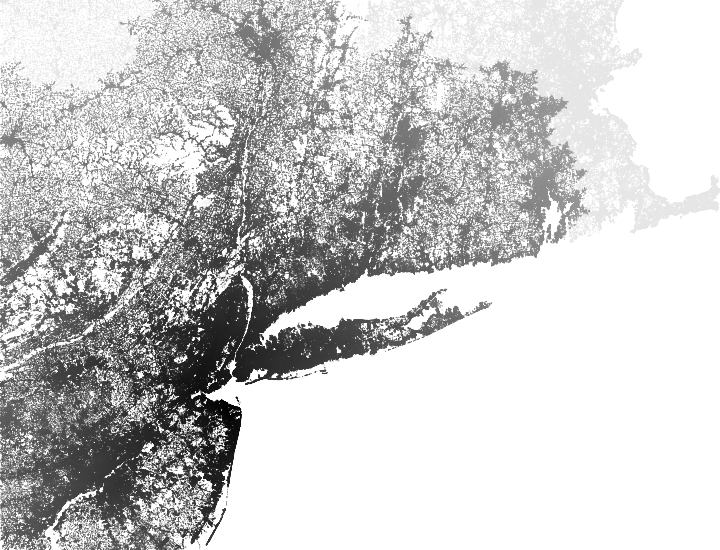
\includegraphics[width=5cm]{figs/incbi-road-ne/singleshot/example-incuni-0.png}%
   }
   
   \subfloat[Replan search]{%
      \centering%
      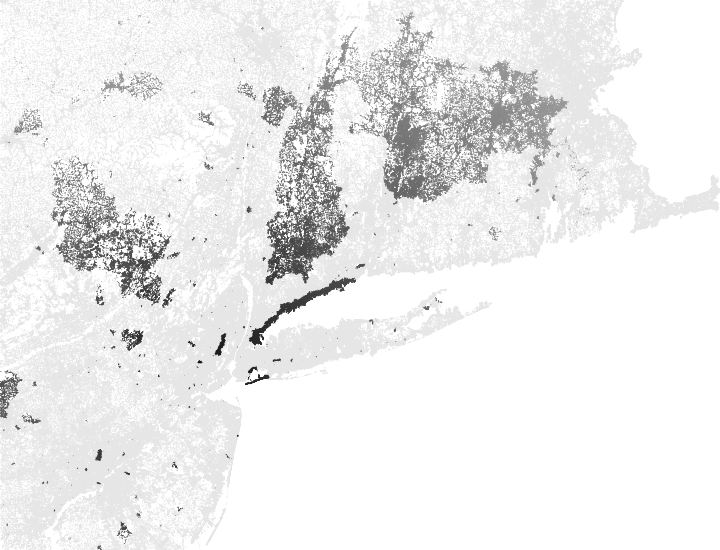
\includegraphics[width=5cm]{figs/incbi-road-ne/singleshot/example-incuni-1.png}%
   }%
   \caption{Initial search: 1,287,897 expansions.
      Replan: 391,122 expansions.}%
   %\label{fig:ibid:example-bidirectional}%
\end{marginfigure}

\subsection{Approximation Completeness}

For bidirectional search,
it's also necessary to be able to prove that you have found
all vertices within a certain distance of the start.
Basically, this is a completeness proof --
if a distance exists below a certain value,
we will have found it.
This is completeness of the approximation,
not of an algorithm per se.

\begin{theorem}
Any vertex $x$ with $d^*(x) < k_{\ms{min}}$
has $d[x] = d^*(x)$.
\label{thm:ibid-dynamicswsffp-complete}
\end{theorem}

\begin{proof}[Proof of Theorem~\ref{thm:ibid-dynamicswsffp-complete}]
We show that $d[x]$ can be both
no less than $d^*(x)$
(Lemma~\ref{lemma:ibid-dynamicswsffp-complete-geq})
and no greater than $d^*(x)$
(Lemma~\ref{lemma:ibid-dynamicswsffp-complete-leq}).
\end{proof}

\begin{lemma}
Any vertex $x$ with $d^*(x) < k_{\ms{min}}$
has $d[x] \geq d^*(x)$.
\label{lemma:ibid-dynamicswsffp-complete-geq}
\end{lemma}

\begin{proof}[Proof of Lemma~\ref{lemma:ibid-dynamicswsffp-complete-geq}]
We show this by contradiction.
Suppose there exists a vertex $x$ with $d^*(x) < k_{\ms{min}}$
for which $d[x] < d^*(x)$.
Then $d[x] < k_{\ms{min}}$,
so $x$ must be consistent.
By Lemma~\ref{lemma:ibid-dynamicswsffp-sound-geq},
we must have $d[x] \geq d^*(x)$.
This contradicts our supposition.
\end{proof}

\begin{lemma}
Any vertex $x$ with $d^*(x) < k_{\ms{min}}$
has $d[x] \leq d^*(x)$.
\label{lemma:ibid-dynamicswsffp-complete-leq}
\end{lemma}

\begin{proof}[Proof of Lemma~\ref{lemma:ibid-dynamicswsffp-complete-leq}]
This proof proceeds in a similar way to that for
Lemma~\ref{lemma:ibid-dynamicswsffp-sound-leq}.
Construct a true shortest path from $s$ to $x$,
with $d^*$-values increasing monotonically from
$d^*(s) = 0$ to $d^*(x)$.
Consider each edge $e_{uv}$ in turn as follows.
Assume that $u$ is consistent,
with $d[u] \leq d^*(u)$.
Note that this is true for the first edge with $u = s$,
since with $0 \leq d^*(x)$,
we have $0 < k_{\ms{min}}$,
so that $s$ must is consistent with $r[s] = d[s] = d^*(s) = 0$.
Since $e_{uv}$ lies on a true shortest path,
we must have $d^*(u) + w(e_{uv}) = d^*(v)$,
and for all edges $d[u] + w(e_{uv}) \geq r[v]$.
Together, this implies that
$d^*(u) - d[u] \leq d^*(v) - r[v]$.
Our assumption that $d[u] \leq d^*(u)$
therefore implies that $r[v] \leq d^*(v)$.
Since $d^*(v) \leq d^*(x)$ and $d^*(x) < k_{\ms{min}}$,
we know that $v$ is consistent,
so we conclude that $d[v] \leq d^*(v)$,
and we can proceed to the next edge on the path.
We end with $v = x$,
so that $d[x] \leq d^*(x)$.
\end{proof}

\subsection{Incremental Bidirectional Search: The Algorithm}

Important: $s$ and $t$ must be distict!

\begin{theorem}
Define $E_{\ms{conn}}$ as the set of all edges $e_{uv}$ such that
$u$ is $s$-consistent with $d[s] \leq k_s$
and $v$ is $t$-consistent with $d[t] \leq k_t$.
If $k_s > 0$, $k_t > 0$,
and
$\min_{e \in E_{\ms{conn}}} \left( d_s[u] + w(e_{uv}) + d_t[v] \right)
   \leq k_s + k_t$,
then the path through $e_{uv}$ is a shortest path.
\label{thm:ibid-sound}
\end{theorem}

\begin{proof}[Proof of Theorem~\ref{thm:ibid-sound}]
We will prove this by contradiction.
Suppose that a path $p'$ exists with
$\mbox{len}(p') < \min_{e \in E_{\ms{conn}}} \left( d_s[u] + w(e_{uv}) + d_t[v] \right)$.
Then it must also be that
$\mbox{len}(p') < k_s + k_t$.
We will consider two cases.

First, consider the case where $k_s > \mbox{len}(p')$,
so that $k_s > d_s^*(t)$.
In this case,
the last edge $e_{ut}'$ on $p'$
has $d_s^*(u') < d_s^*(t) < k_s$;
by Theorem~\ref{thm:ibid-dynamicswsffp-complete},
$u'$ is therefore $s$-consistent with $d_s[u'] = d_s^*(u')$.
In addition,
since $k_t > 0$,
$t$ must be $t$-consistent with $d_t[t] = 0$.
Therefore,
it follows that $d_s^*(u') + w(e_{ut}') < d_s[u'] + w(e_{ut}')$,
which contradicts the supposition.

In the second case with $k_s \leq \mbox{len}(p')$,
identify on $p'$ the edge $e'_{uv}$ adjoining the vertices $u'$, $v'$
such that $d_s^*(u') < k_s \leq d_s^*(v')$.
(Since $k_s > 0$, this edge will exist.)
Since $d_s^*(u') < k_s$,
by Theorem~\ref{thm:ibid-dynamicswsffp-complete},
$u'$ is therefore $s$-consistent with $d_s[u'] = d_s^*(u')$.
Consider our supposition that
$d_s^*(u') + w(e_{uv}') + d_t^*(v') < k_s + k_t$.
Since $d_s^*(u') + w(e_{uv}') = d_s^*(v')$
and $k_s \leq d_s^*(v')$,
it follows that
$d_t^*(v') < k_t$.
Therefore,
by Theorem~\ref{thm:ibid-dynamicswsffp-complete},
$v'$ is $t$-consistent with $d_t[v'] = d_t^*(v')$.
As a consequence,
the edge $e'_{uv}$ must be in $E_{\ms{conn}}$.
Therefore,
$d_s^*(u') + w(e_{uv}') + d_t^*(v')
   < d_s[u'] + w(e_{uv}') + d_t[v']$,
which is a contradiction.
\end{proof}

\begin{marginfigure}%
   \centering%
   \subfloat[Initial search]{%
      \centering%
      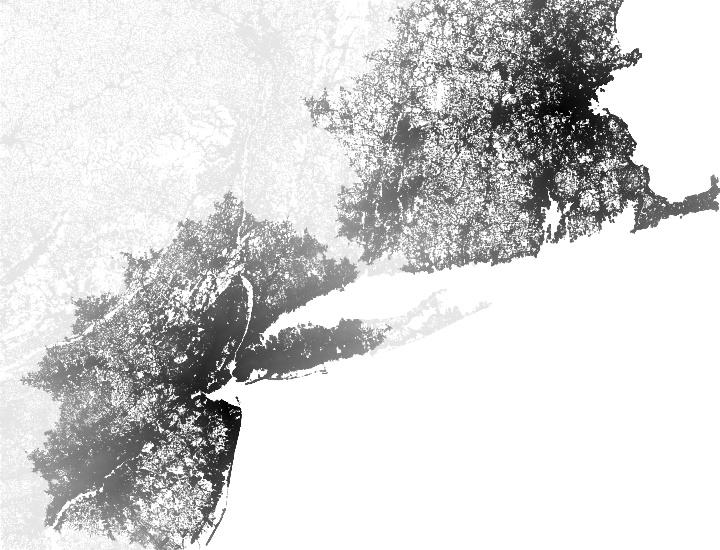
\includegraphics[width=5cm]{figs/incbi-road-ne/singleshot/example-incbi-0.png}%
   }
   
   \subfloat[Replan search]{%
      \centering%
      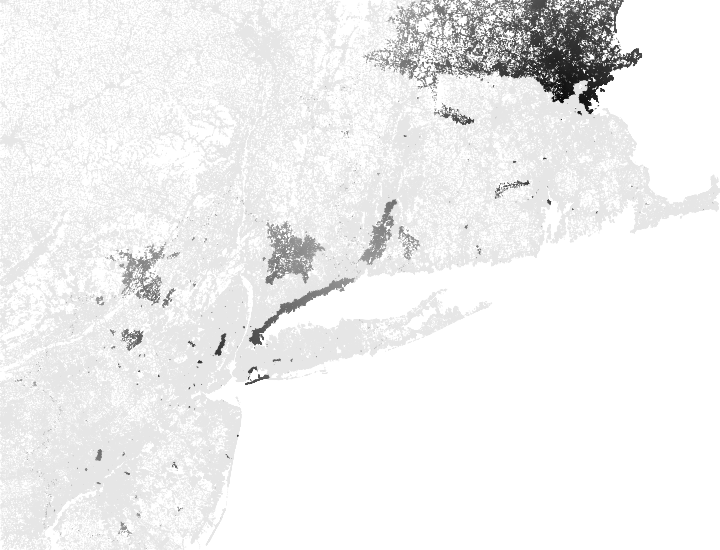
\includegraphics[width=5cm]{figs/incbi-road-ne/singleshot/example-incbi-1.png}%
   }%
   \caption{Initial search: 1,181,616 expansions.
      Replan: 262,422 expansions.}%
   %\label{fig:ibid:example-bidirectional}%
\end{marginfigure}






\subsection{IBiD}

The main outline of IBiD is given in Algorithm~\ref{alg:ibid}.
IBiD conducts two independent DynamicSWSF-FP searches
(Algorithm~\ref{alg:ibid-two-dynamicswsffps}).

\begin{algorithm}[t]
   \caption{IBiD Outline}
   \label{alg:ibid}
   \begin{algorithmic}[1]
      \Procedure {Main} {\,}
         \State $\mbox{\sc InitializeSource}(); \; \mbox{\sc InitializeTarget}()$
         \State $Q_c \gets \emptyset$
            \Comment $\mbox{ key for } (u,v): d_s(u) + w(u,v) + d_t(v)$
         \Loop
            \While {not $\mbox{\sc TerminationCondition}()$}
               \If {$Q_s.\mbox{TopKey} < Q_t.\mbox{TopKey}$}
                     \Comment prioritize arbitrarily
                  \State $\mbox{\sc ProcessSourceQueue}(u)$
               \Else
                  \State $\mbox{\sc ProcessTargetQueue}(u)$
               \EndIf
               \State Ensure $(u,v) \in Q_c$ iff
                  $u \neq Q_s$, $v \neq Q_t$, key $\neq \infty$
            \EndWhile
            \State $(u_c,v_c) \gets Q_c.\mbox{Top}$
            \State $\pi \gets
               ( \mbox{walk } d_s \mbox{ from } u_c \mbox{ to } s )
               \cup
               ( \mbox{walk } d_t \mbox{ from } v_c \mbox{ to } t )$
            \State wait for edges $(u,v) \in E_{\ms{delta}}$ with changed weights $w(u,v)$
            \State $\mbox{\sc NotifyWeightChanges}(E_{\ms{delta}})$
         \EndLoop
      \EndProcedure
      \Function {TerminationCondition} {\,}
         \State $(u_c,v_c) \gets Q_c.\mbox{TopKey}$
            \Comment return False if $Q_c$ empty
         \If {$Q_s.\mbox{TopKey} + Q_t.\mbox{TopKey} < d_s(u_c) + w(u_c,v_c) + d_t(v_c)$}
            \State \Return False
         \EndIf
         \If {$Q_s.\mbox{TopKey} < d_s(u_c)$
               \mbox{\bf or} $Q_t.\mbox{TopKey} < d_t(v_c)$}
            \State \Return False
         \EndIf
         \State \Return True
      \EndFunction
      \Procedure {NotifyWeightChanges} {$E_{\ms{delta}}$}
         \ForAll {$(u,v) \in E_{\ms{delta}}$}
            \State $\mbox{\sc UpdateSourceDistance}(v)$
            \State $\mbox{\sc UpdateTargetDistance}(u)$
         \EndFor
         \State Ensure $(u,v) \in Q_c$ iff
            $u \neq Q_s$, $v \neq Q_t$, key $\neq \infty$
      \EndProcedure
   \end{algorithmic}
\end{algorithm}

{\floatevery{algorithm}{\setlength\hsize{16.85cm}}
\begin{algorithm}[t]
   \caption{As a bidirectional algorithm,
      IBiD conducts two independent DynamicSWSF-FP searches,
      one computing distance from the source vertex,
      and the other computing distance to the target vertex.}
   \label{alg:ibid-two-dynamicswsffps}
   \begin{minipage}[t]{8.2cm}
      \begin{algorithmic}[1]
         \Procedure {InitializeSource} {\,\!}
            \ForAll {$v \in V$}
               \State $d_s(v) \gets \infty; \;\; r_s(v) \gets \infty$
            \EndFor
            \State $r_s(s) \gets 0$
            \State $Q_s \gets \{ s \}$
               \Comment $\mbox{ key for } v: \min\big(r_s(v),d_s(v)\big)$
            \State $\mbox{\sc ProcessSourceQueue}()$
         \EndProcedure
         \Procedure {UpdateSourceDistance} {$v$}
            \If {$v \neq s$}
               \State $r_s(v) \gets \displaystyle\min_{u \in \mbox{\scriptsize Pred}(v)}
                  \big( d_s(u) + w(u,v) \big)$
            \EndIf
            \State Ensure $v \in Q_s$ iff $d_s(v) \neq r_s(v)$
         \EndProcedure
         \Procedure {ProcessSourceQueue} {\,\!}
            \State $u \gets Q_s.\mbox{Pop}()$
            \If {$r_s(u) < d_s(u)$}
                  \Comment over-consistent
               \State $d_s(u) \gets r_s(u)$
               \ForAll {$v \in \mbox{Succ}(u)$}
                  \State $\mbox{\sc UpdateSourceDistance}(v)$
               \EndFor
            \Else
                  \Comment under-consistent
               \State $d_s(u) \gets \infty$
               \ForAll {$v \in \mbox{Succ}(u) \cup u$}
                  \State $\mbox{\sc UpdateSourceDistance}(v)$
               \EndFor
            \EndIf
         \EndProcedure
         \algstore{ibid-two-dynamicswsffps}
      \end{algorithmic}
   \end{minipage}
   \quad
   \begin{minipage}[t]{8.2cm}
      \begin{algorithmic}[1]
         \algrestore{ibid-two-dynamicswsffps}
         \Procedure {InitializeTarget} {\,\!}
            \ForAll {$v \in V$}
               \State $d_t(v) \gets \infty; \;\; r_t(v) \gets \infty$
            \EndFor
            \State $r_t(t) \gets 0$
            \State $Q_t \gets \{ t \}$
               \Comment $\mbox{ key for } v: \min\big(r_t(v),d_t(v)\big)$
            \State $\mbox{\sc ProcessTargetQueue}()$
         \EndProcedure
         \Procedure {UpdateTargetDistance} {$u$}
            \If {$u \neq t$}
               \State $r_t(u) \gets \displaystyle\min_{v \in \mbox{\scriptsize Succ}(u)}
                  \big( w(u,v) + d_t(v) \big)$
            \EndIf
            \State Ensure $u \in Q_t$ iff $d_t(u) \neq r_t(u)$
         \EndProcedure
         \Procedure {ProcessTargetQueue} {\,\!}
            \State $v \gets Q_t.\mbox{Pop}()$
            \If {$r_t(v) < d_t(v)$}
                  \Comment over-consistent
               \State $d_t(v) \gets r_t(v)$
               \ForAll {$u \in \mbox{Pred}(v)$}
                  \State $\mbox{\sc UpdateTargetDistance}(u)$
               \EndFor
            \Else
                  \Comment under-consistent
               \State $d_t(v) \gets \infty$
               \ForAll {$u \in \mbox{Pred}(v) \cup v$}
                  \State $\mbox{\sc UpdateTargetDistance}(u)$
               \EndFor
            \EndIf
         \EndProcedure
      \end{algorithmic}
   \end{minipage}
\end{algorithm}
} % floatevery width adjustment

\section{Heuristic Search}
\label{sec:ibid:heuristic}

Heuristic methods such as the Graph Traverser
\citep{doran1966graphtraverser} were originally
applied to pathfinding problems in order to find non-optimal
solutions more economically.
These unidirectional methods proceed similarly to Dijkstra's algorithm,
but instead of prioritizing {\sc Open} vertices
based on their source distance $d_s$,
they use a target-directed heuristic function $h_t$.
Hart, Nilsson, and Raphael \citep{hart1968astar} discovered that
these approaches can be combined ($d_s + h_t$) to yield
an admissible algorithm (A*) for the shortest-path problem,
as long as $h_t$ meets certain conditions.

\paragraph{Example problem.}
\begin{marginfigure}%
   \centering%
   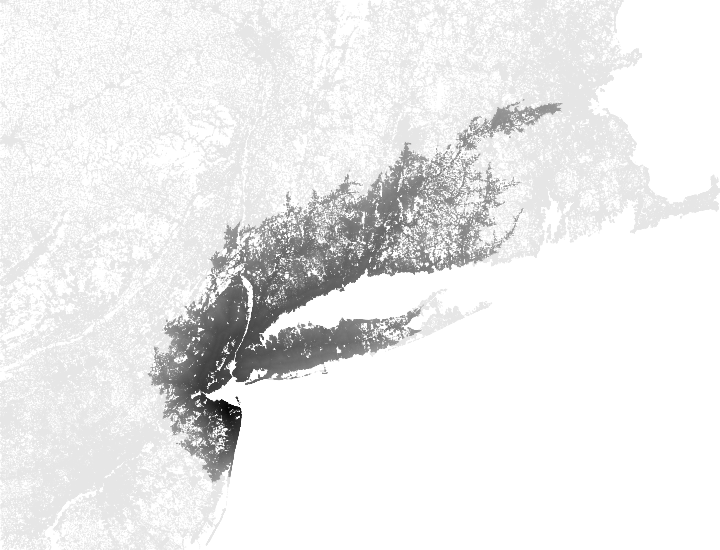
\includegraphics[width=5cm]{figs/incbi-road-ne/singleshot/example-astar.png}%
   \caption{A* search.
      532,880 expansions.}%
   \label{fig:ibid:example-astar}%
\end{marginfigure}
See Figure~\ref{fig:ibid:example-astar}.
For the purpose of calculating vertex heuristics,
geographic coordinates were projected onto a 2D plane using the
scale at the midpoint latitude ($41.25^\circ$)
resulting in a projecting error of less than 0.3\%.
The maximum transit speed is 30.11 m/s.

Attempts to provide a bidirectional algorithm which incorporates
heuristics generally take one of three approaches.
\cdnote{I need to deep-dive here to write this correctly.}

First,
front-to-front methods
could evaluate the heuristic between all pairs in the two
{\sc Open} sets.
Expensive.

Second,
perform two heuristic-informed searches,
and account for the connection problem via a complex
termination condition.
Not necessarily efficient.
(Pohl cites Berge?)
Missile analogy.

Third,
waste (same heuristic function).

Concept of waste \citep{pohl1969bidirectional}.
I think this subsumes A*.

Talk about the 94 paper \citep{ikeda1994betterroutes}
expressing A* as a search on
the waste graph.

As a potential function.
Also Goldberg \citep{goldberg2005spexternalmemory}.

To integrate: \citep{dechter1984bfsastaropt}.

\paragraph{Example problem.}
\begin{marginfigure}%
   \centering%
   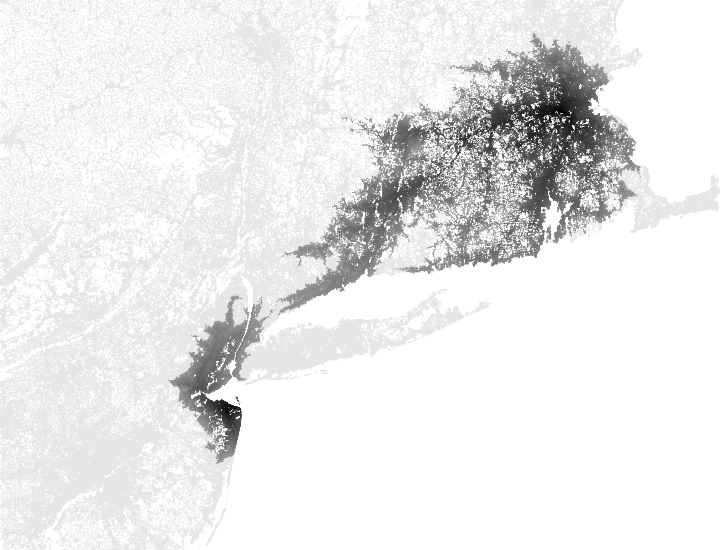
\includegraphics[width=5cm]{figs/incbi-road-ne/singleshot/example-heurbidijkstra.png}%
   \caption{Bidirectional A* search.
      515,588 expansions.}%
   \label{fig:ibid:example-heurbidijkstra}%
\end{marginfigure}
See Figure~\ref{fig:ibid:example-heurbidijkstra}.

\subsection{The Zero-Weight Problem}

Talk about how a perfect potential leads to zero waste,
which breaks incremental search.
This motivates the lexocraphically sorted key approach.

\subsection{Incremental Heuristic Search}

Apply waste to incremental search to get
incremental heuristic search.

Lifelong Planning A* \citep{koenig2004lpastar}.

\section{Other Stuff}

\subsection{Examples}

See Figure~\ref{fig:incbi-lpastar-fig1-heurchange}
and Figure~\ref{fig:incbi-lpastar-fig1}.

\begin{figure}
   \centering%
   
   \includegraphics{build/incbi-lpastar-fig1/lpastar-heurnone-original}%
   \;\;%
   \includegraphics{build/incbi-lpastar-fig1/incbi-heurnone-original}%
   
   \vspace{0.2cm}
   
   \includegraphics{build/incbi-lpastar-fig1/lpastar-heurhalf-original}%
   \;\;%
   \includegraphics{build/incbi-lpastar-fig1/incbi-heurhalf-original}%
   
   \vspace{0.2cm}
   
   \includegraphics{build/incbi-lpastar-fig1/lpastar-heurfull-original}%
   \;\;%
   \includegraphics{build/incbi-lpastar-fig1/incbi-heurfull-original}%
   
   \caption{Illustration of behavior of IBiD on a single
      (non-incremental) shortest path problem.
      At left, IBiD uses the unidirectional start-side expansion
      strategy.
      At right, IBiD uses the bidirectional distance-balanaced
      expansion strategy.
      Start and goal heuristic functions are available;
      the unidirectional search uses a potential function based
      on the goal heuristic,
      and the bidirectional search a potential function using
      the average heuristic.
      IBiD is run with three different potential function weights:
      0.0 (top), 0.5 (middle), and 1.0 (bottom).
      IBiD therefore preforms equivalently to
      Dijkstra's algorithm (top-left),
      Bidirectional Dijkstra's (top-right),
      A* (bottom-left),
      and Bidirectional A* (bottom-right).}
   \label{fig:incbi-lpastar-fig1-heurchange}
\end{figure}

\begin{figure}
   \centering%
   
   \includegraphics{build/incbi-lpastar-fig1/lpastar-heurfull-original}%
   \;\;%
   \includegraphics{build/incbi-lpastar-fig1/lpastar-heurfull-changed}%
   
   \vspace{0.2cm}
   
   \includegraphics{build/incbi-lpastar-fig1/incbi-heurfull-original}%
   \;\;%
   \includegraphics{build/incbi-lpastar-fig1/incbi-heurfull-changed}%
   
   \caption{IBiD with only source-side expansions and a goal-side
      heuristic (top) proceeds identically to Lifelong Planning A*,
      performing 37 expansions on the original world (left)
      followed by 18 expansions over 14 vertices on the chanced
      world (right).
      IBiD with distance-balanced expansions and an average
      potential (bottom)
      performs 30 expansions on the original world
      followed by 18 expansions over 15 vertices on the changed
      world.}
   \label{fig:incbi-lpastar-fig1}
\end{figure}

\begin{figure*}
   \centering%
   
   \begin{tabular}{ccc}
      \specialcell{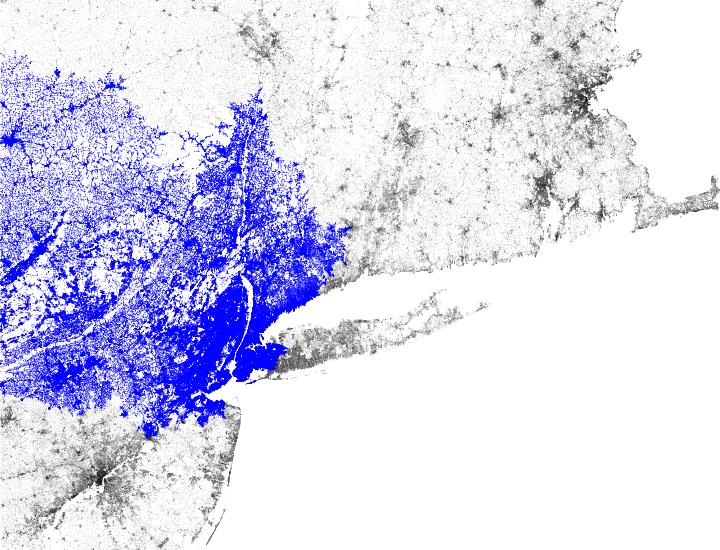
\includegraphics[width=5cm]{figs/incbi-road-ne/singleshot/pgoalnone-balfwd.png}\\556,209 expansions}
      &
      \specialcell{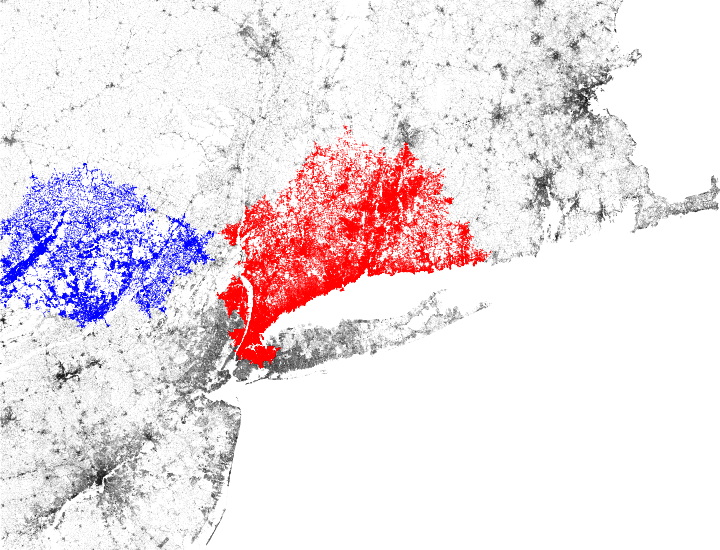
\includegraphics[width=5cm]{figs/incbi-road-ne/singleshot/pavgnone-baldist.png}\\319,938 expansions}
      &
      \specialcell{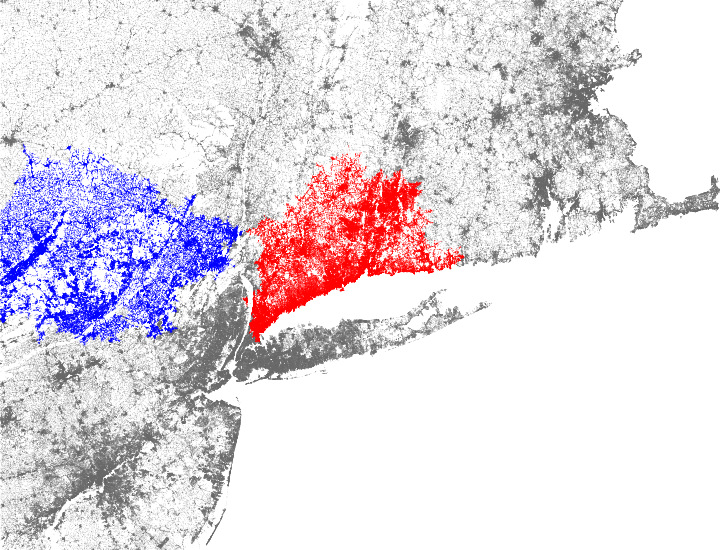
\includegraphics[width=5cm]{figs/incbi-road-ne/singleshot/pavgnone-balcard.png}\\281,413 expansions}
      \vspace{0.3cm}
      \\
      \specialcell{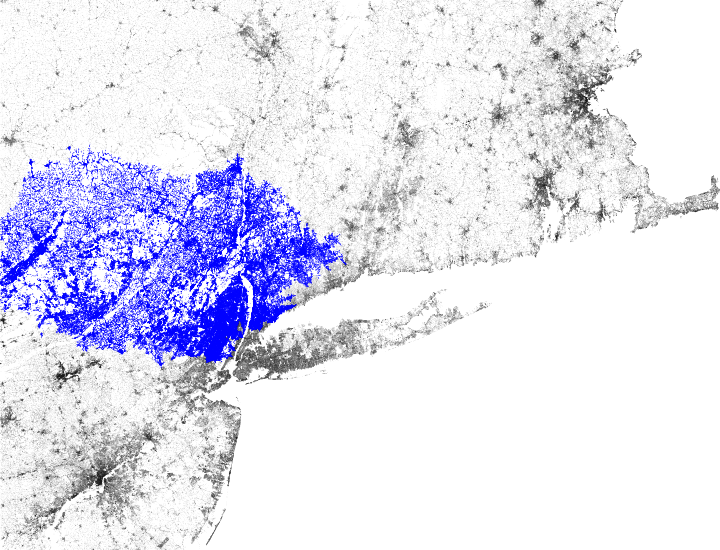
\includegraphics[width=5cm]{figs/incbi-road-ne/singleshot/pgoalhalf-balfwd.png}\\297,414 expansions}
      &
      \specialcell{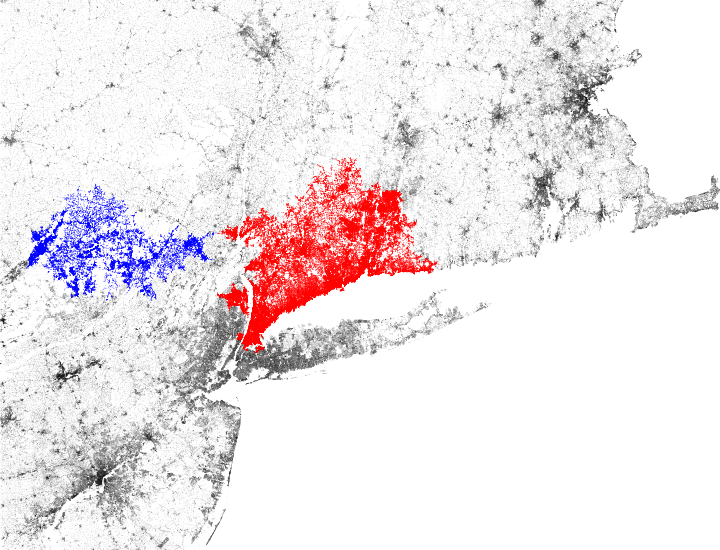
\includegraphics[width=5cm]{figs/incbi-road-ne/singleshot/pavghalf-baldist.png}\\206,625 expansions}
      &
      \specialcell{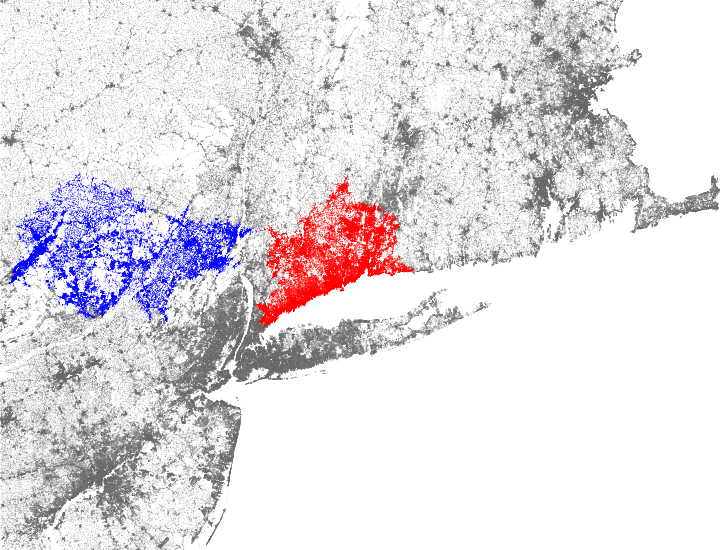
\includegraphics[width=5cm]{figs/incbi-road-ne/singleshot/pavghalf-balcard.png}\\178,929 expansions}
      \vspace{0.3cm}
      \\
      \specialcell{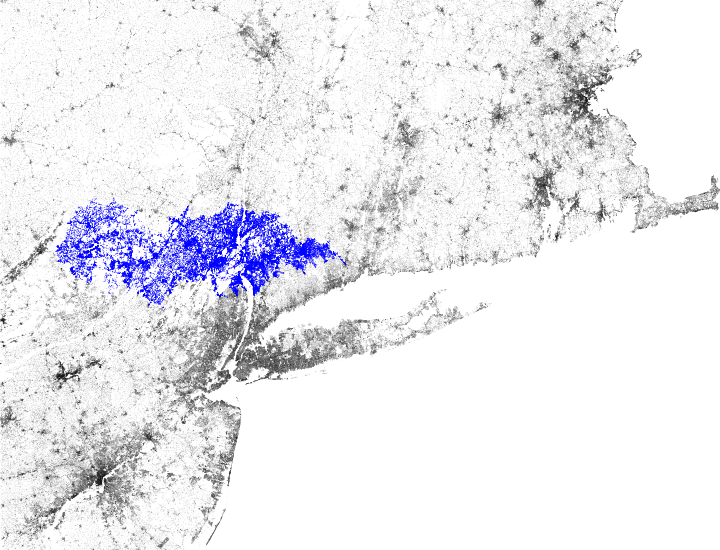
\includegraphics[width=5cm]{figs/incbi-road-ne/singleshot/pgoalfull-balfwd.png}\\82,915 expansions}
      &
      \specialcell{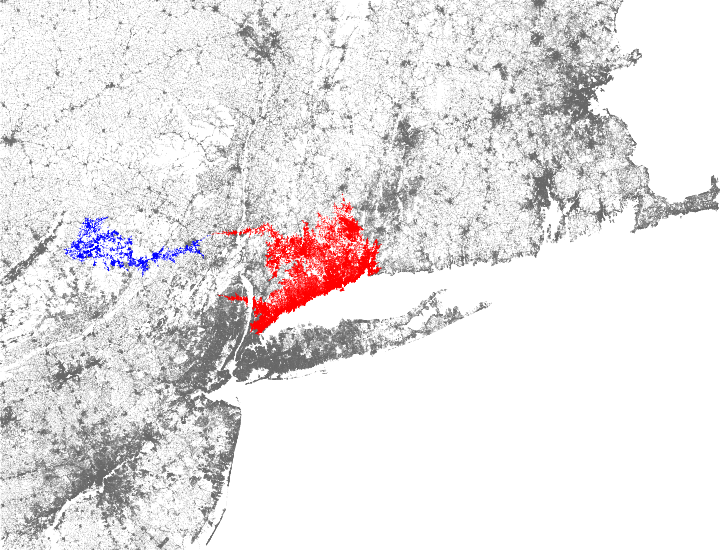
\includegraphics[width=5cm]{figs/incbi-road-ne/singleshot/pavgfull-baldist.png}\\95,759 expansions}
      &
      \specialcell{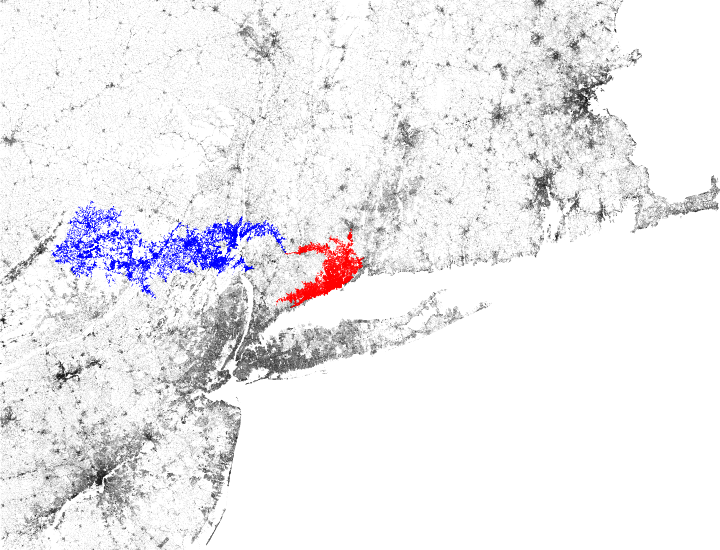
\includegraphics[width=5cm]{figs/incbi-road-ne/singleshot/pavgfull-balcard.png}\\69,218 expansions}
      \vspace{0.5cm}
   \end{tabular}
   
   \caption{Comparison between various heuristic strengths and
      balancing strageties on a single-pair road network problem.
      A path with shortest transit time is sought.
      The heuristic strength varies from no heuristic (top)
      to a full-strength heuristic (bottom).
      At left, a foward-only balancer is used, so that the
      top-left is equivalent to Dijkstra's algorithm,
      and the bottom-left is equivalent to A*.
      The middle column uses a balanced distance strategy.
      The right column uses a balanced cardinality strategy.}
   \label{fig:incbi-road-ne}
\end{figure*}

\subsection{LazySP Selector Experiments}

\begin{figure}
   \centering
   \includegraphics{build/incbi-sq/all-even}
   \caption{Across a selection of articulated robot planning instances,
      using the Even edge selector.
      Algorithms are
      \protect\tikz{\protect\node[fill=black!30,draw=black,postaction={pattern=north west lines}]{};}\;LPA*,
      \protect\tikz{\protect\node[fill=black!20,draw=black]{};}\;IBiD,
      and \protect\tikz{\protect\node[fill=black!30,draw=black,postaction={pattern=north east lines}]{};}\;Reverse LPA*.
      Results shown are cumulative search time.
      }
\end{figure}

\begin{figure}
   \centering
   \includegraphics{build/incbi-road-ne/stats}
   \caption{Road network incremental results.
      Algorithms are
      \protect\tikz{\protect\node[fill=black!30,draw=black,postaction={pattern=north west lines}]{};}\;LPA*,
      \protect\tikz{\protect\node[fill=black!20,draw=black]{};}\;IBiD,
      and \protect\tikz{\protect\node[fill=black!30,draw=black,postaction={pattern=north east lines}]{};}\;Reverse LPA*.
      }
\end{figure}

\begin{figure}
   \centering
   \includegraphics{build/incbi-sq/herbbin0}
   
   \includegraphics{build/incbi-sq/herbbin0-lambda}
   \caption{Problem: \texttt{herbbin0}.
      Lines are:
      \protect\tikz{\protect\draw[thick] (0,0) -- (0.15,0.15);} no heuristic,
      \protect\tikz{\protect\draw[densely dashed] (0,0) -- (0.15,0.15);} start heuristic,
      \protect\tikz{\protect\draw[densely dashdotted] (0,0) -- (0.15,0.15);} avg heuristic,
      \protect\tikz{\protect\draw[densely dotted] (0,0) -- (0.15,0.15);} goal heuristic.
      }
\end{figure}

\begin{figure*}
   \centering
   \includegraphics{build/incbi-sq/herbbookshelf0}
   \includegraphics{build/incbi-sq/herbbookshelf1nom}
   
   \includegraphics{build/incbi-sq/herbbookshelf0-lambda}
   \includegraphics{build/incbi-sq/herbbookshelf1nom-lambda}
   \caption{Problems: \texttt{herbbookshelf0} (left), texttt{herbbookshelf1nom} (right).}
\end{figure*}

\begin{figure*}
   \centering
   \includegraphics{build/incbi-sq/workcellef}
   \includegraphics{build/incbi-sq/workcellij}
   
   \includegraphics{build/incbi-sq/workcellef-lambda}
   \includegraphics{build/incbi-sq/workcellij-lambda}
   \caption{Problems: \texttt{workcellef} (left), \texttt{workcellij} (right).}
\end{figure*}

\subsection{Implementation Details}

Other implementations:
\citep{alberts1998softwaredynamicgraph}.
